\subsection{\en{Thread Affinity}}
\subparagraph{}
\emph{\en{Thread Affinity}} είναι μια ευρύτερη έννοια που περιλαμβάνει την βελτιστοποίηση του χρόνου εκτέλεσης ενός προγράμματος, μέσω βελτιστοποιήσεων στο εύρος ζώνης μνήμης, τη ν αποφυγή καθυστέρησης μνήμης ή της  καθυστέρησης χρήσης προσωρινής μνήμης.

To \emph{\en{OpenMP 4.0}} εισάγει ένα σύνολο οδηγιών για την υποστήριξη του \emph{\en{thread affinity}}\cite{thread_affinity}. Η πλειοψηφία πλέον των μηχανημάτων βασίζονται στην \emph{\en{cc-NUMA}} αρχιτεκτονική. Ο λόγος που αυτό το σύστημα μνήμης έγινε κυρίαρχο, είναι η συνεχής αύξηση του αριθμού των επεξεργαστών. Η μονολιθική διασύνδεση μνήμης με σταθερό εύρος ζώνης μνήμης θα αποτελούσε πρόβλημα στην ραγδαία αύξηση των επεξεργαστών.

Στη \emph{\en{cc-NUMA}} αρχιτεκτονική κάθε υποδοχή συνδέεται με ένα υποσύνολο της συνολικής μνήμης του συστήματος. Μία διασύνδεση ενώνει τα υποσύνολα μεταξύ τους και δημιουργεί την εικόνα ενιαιας μνήμης στον χρήστη. Ενα τέτοιο σύστημα είναι ευκολότερο να επεκταθεί.

Το πλεονέκτημα της διασύνδεσης είναι ότι η εφαρμογή έχει πρόσβαση σε όλη την μνήμη του συστήματος, ανεξάρτητα από το που βρίσκονται τα δεδομένα. Ωστόσο, πλεον ο χρόνος πρόσβασης σε αυτά δεν ειναι ο σταθερός καθώς εξαρτάται από τη θέση τους στη μνήμη.


\begin{figure}[h]
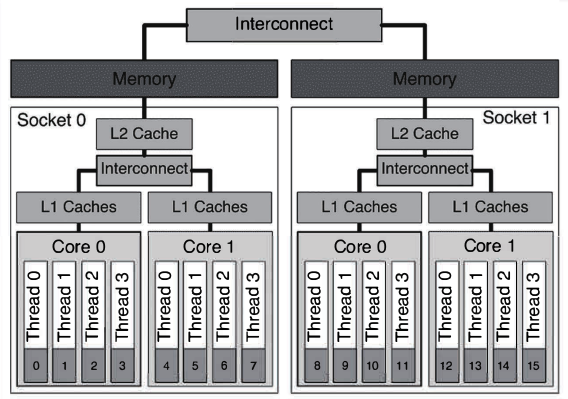
\includegraphics[width=0.75\textwidth]{numa}
\centering
\captionsetup{justification=centering, singlelinecheck=false}
	\caption{Αρχιτεκτονική \en{cc-NUMA}\cite{thenextstep152}}
\label{fig:numa}
\end{figure}

